\documentclass[a4paper,14pt]{extarticle}
\usepackage[top=2cm, bottom=2cm, left=2cm, right=2cm]{geometry}
\usepackage[parfill]{parskip}
\usepackage{graphicx}
\usepackage{tikz}
\usepackage{amsmath}
\begin{document}
\begin{center}
\LARGE{MECH 4450 Term Project Report}\\\vspace{1em}
\Large{Project 2 (Static structure)}\\\vspace{1em}
\Large{Kong Xiangzhou 20026414}\\\vspace{1em}
\end{center}
\section{Introduction}
\subsection{Description of the problem}
The cable anchor is a component at the end of the guy wire that helps to anchor the guyed tower as the picture below shows. It is widely used in engineering structures, such as broadcast transmission towers, bridges and so on. The problem is to analyze the load of the anchor, and to optimize the design.

\begin{center}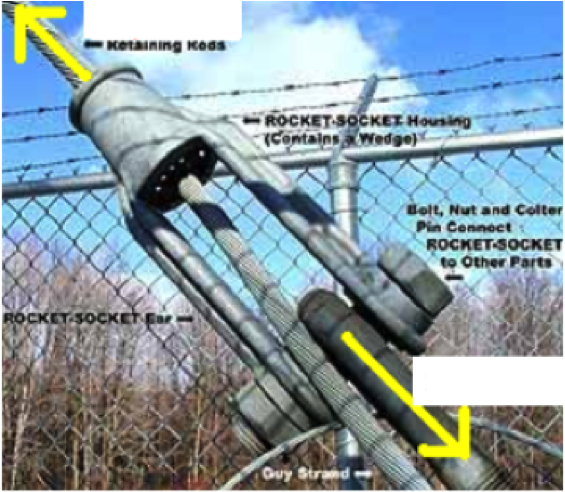
\includegraphics[width=0.5\textwidth]{DESCRIPTION.png}\end{center}

In the analysis part, it is need to find out the points where failure is most possible to happen. In other words, the place where maximum local stress occurs. The design part will be discussed below.

Commercial finite element analysis software suite ANSYS will be used.
\subsection{Design objectives}
\begin{itemize}
\item The safety factor is required to be at least 2. 
\item The weight of the structure should be minimized.
\item Dimensions should be adjusted in a way that other components (the guy wire and the bolt) will also have a good safefy factor, and the connection between the anchor and other components are safe enough. For example, decrease $D2$ may increase the safety factor and reduce the weight of the anchor itself, but it will reduce the safety factor of the bolt significantly.
\end{itemize}

\subsection{Conditions}
The material used to build the cable anchor will be structural steel.

Some dimensions are fixed.  $H9=25cm$, $V7=6cm$, $D1 = 6cm$.

The cable anchor will be loaded with a axial force of $2\times10^5 N$. On one side, the force will be exerted on the guy wire via a cylindrical surface in a form of frictional force. It can be treated as fixed support. One the other hand, the force is balanced using a bolt put through two holes. Bearing load can be assumed for the situation.

Symmetrical model can be assumed. 
\section{Program modelling}
\subsection{Geometry}
The top view of original design is shown below:

\begin{center}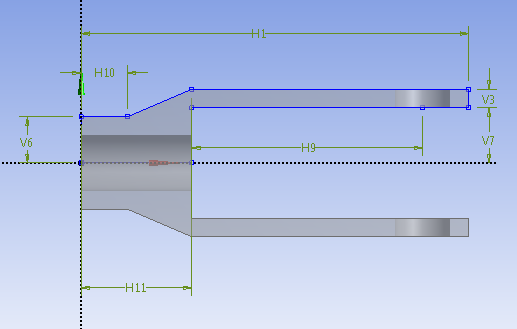
\includegraphics[width=0.75\textwidth]{2D_ORIGIN.png}\end{center}

Where $H1=42cm$, $H10=5cm$, $H11=12cm$, $H9=25cm$, $V3=2cm$, $V6=5cm$, $V7=6cm$, diameters of all holes are $6cm$.

It is resembled as below:

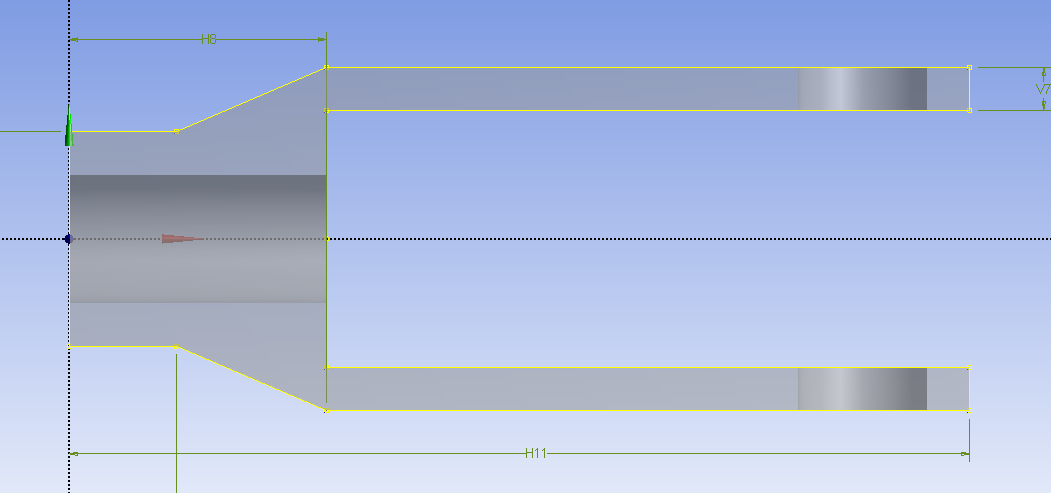
\includegraphics[width=\textwidth]{2D_S_01.PNG}

The 3D model built is then as below, where the height of the component is assumed to be $10 cm$:

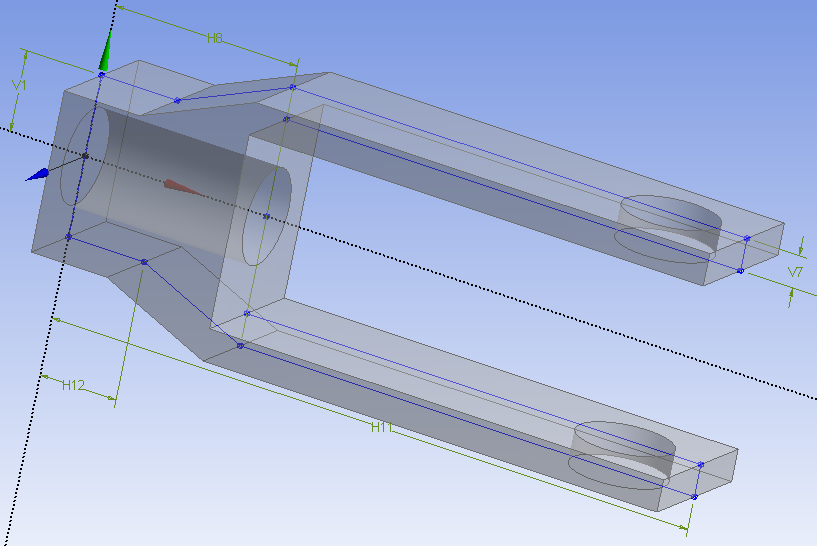
\includegraphics[width=\textwidth]{3D_S_01.PNG}
\section{Boundary conditions}
The boundary conditions are the loads, where symmetric properties on both axis can be assumed.

On the side of the guy wire, it can be treated as fixed support. One the other side, bearing load can be assumed to be each $1\times10^5 N$, and excerted at the wholes. See the parts below for a fihure demonstrating it.
\section{Parameters to optimize}
Only the dimensions marked on the provided figure will be optimized. The topology of the anchor will not be changed. In other words, the optimization will be limited to changing the numbers provided.

To make optimization easier, another set of parameters will be used (note that P6 is not used as the dimension is fixed):

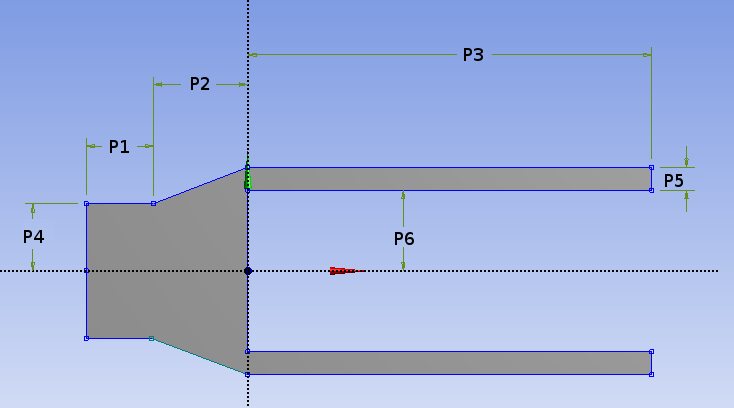
\includegraphics[width=\textwidth]{singleParam/NEW_DIM.PNG}

\begin{align*}
P1 &= H10\\
P2 &= H11-H10\\
P3 &= H1-H11\\
P4 &= V6\\
P5 &= V3\\
P7 &= HEIGHT / 2\\
P8 &= D2
\end{align*}

These parameters will be used in the optimization part of this report.
\section{FEM analysis}
\subsection{Mesh setup}
As this is a 3D model, tetrahedron shape of elements will be used.

For the mesh, two refinements are added as below, where the first one (\textit{Refinement}) is for the cylindrical surface of loading, and the second one (\textit{Refinement 2}) is for the sharp edges of 90 degree where stress concentration might occur.

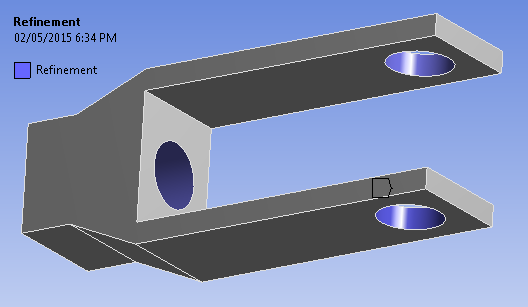
\includegraphics[width=0.5\textwidth]{REF1.PNG}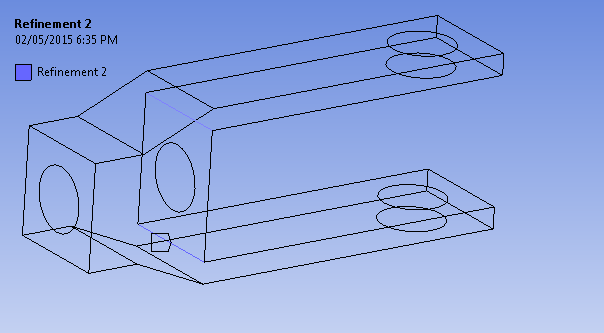
\includegraphics[width=0.5\textwidth]{REF2.PNG}

The overall mesh with a size of $2cm$ is shown below:

\includegraphics[width=0.5\textwidth]{{MESH_0.02}.PNG}\includegraphics[width=0.5\textwidth]{{MESH_0.02F}.PNG}
\subsection{Boundary conditions setup}
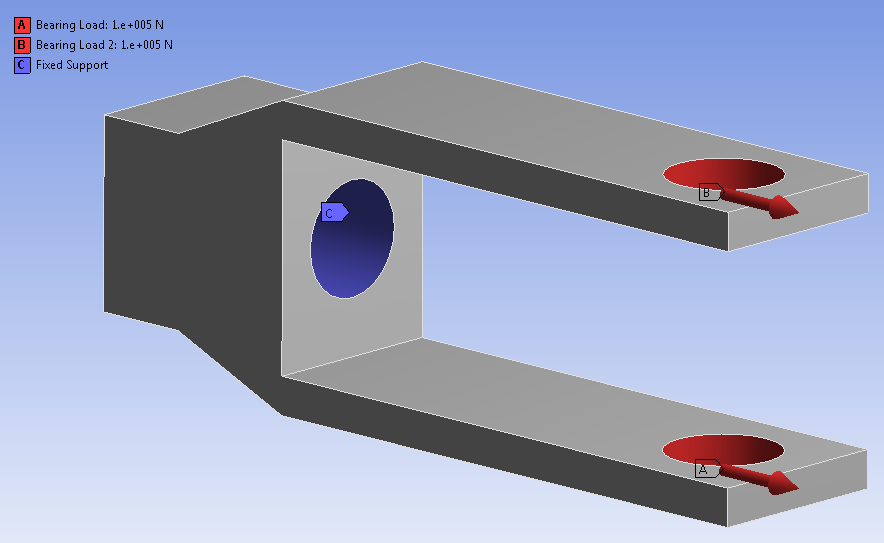
\includegraphics[width=\textwidth]{Model.PNG}
\subsection{Results}
As uniform material is assumed, the local safety factor would be proportional to the local principle stress.

\begin{center}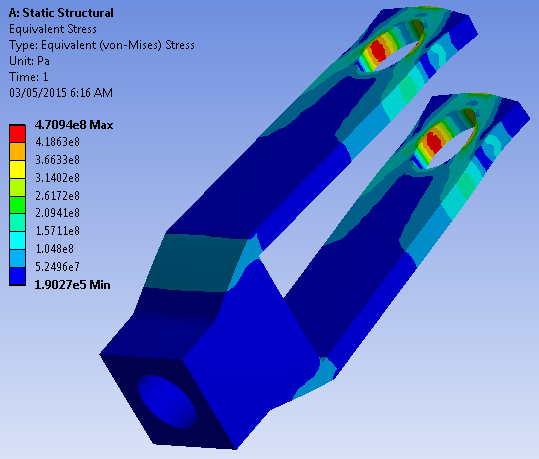
\includegraphics[width=0.75\textwidth]{STRESS_DEFAULT.PNG}\end{center}

We can clear see that the maximum stress is at the four symmetric points: the side end of the wholes. They are exactly the points where failure is most possible to happen.  An enlarged figure below shows it better:

\begin{center}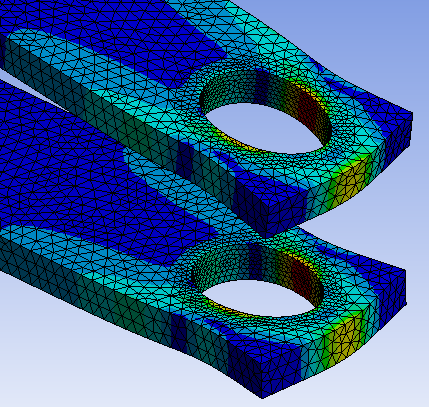
\includegraphics[width=0.5\textwidth]{LOCAL_STRESS.PNG}\end{center}

The local safety factors are shown below:

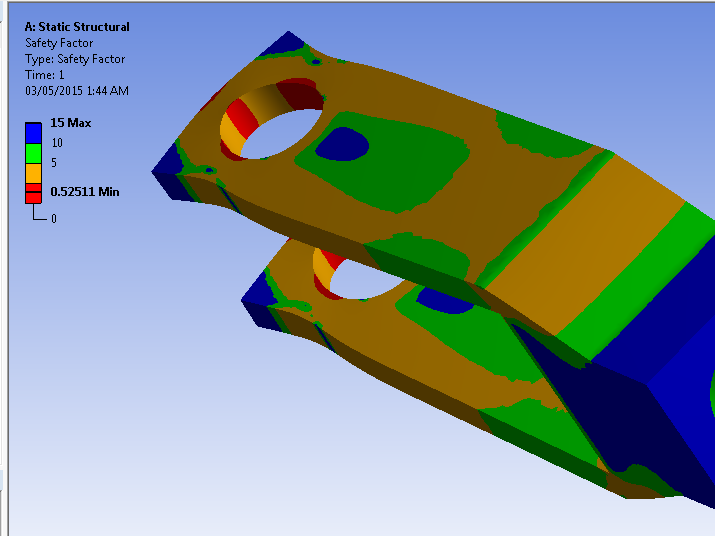
\includegraphics[width=\textwidth]{SF_1.PNG}

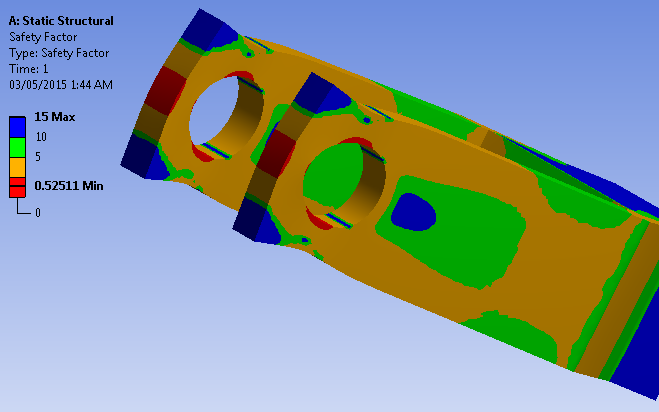
\includegraphics[width=\textwidth]{SF_2.PNG}

Clearly, as the minimum safety factor is around 0.5, the original design does not meet the requirements.

\subsection{Convergence study}
For convergence study, mesh sizes of  $3cm$, $2cm$, $1.5cm$m $1cm$, $0.8cm$ and $0.65cm$ are used. The mesh of minimum ($0.65cm$) and maximum ($3cm$) mesh size are shown below:

\includegraphics[width=0.5\textwidth]{{MESH_0.0065}.PNG}\includegraphics[width=0.5\textwidth]{{MESH_0.03}.PNG}

The results for principle stresses are below, listed in size-decreasing order.

\includegraphics[width=0.5\textwidth]{{STRESS_0.03}.PNG}\includegraphics[width=0.5\textwidth]{{STRESS_0.02}.PNG}
\includegraphics[width=0.5\textwidth]{{STRESS_0.015}.PNG}\includegraphics[width=0.5\textwidth]{{STRESS_0.01}.PNG}
\includegraphics[width=0.5\textwidth]{{STRESS_0.008}.PNG}\includegraphics[width=0.5\textwidth]{{STRESS_0.0065}.PNG}

The results for deformations are below, listed in size-decreasing order.

\includegraphics[width=0.5\textwidth]{{DEFORM_0.03}.PNG}\includegraphics[width=0.5\textwidth]{{DEFORM_0.02}.PNG}
\includegraphics[width=0.5\textwidth]{{DEFORM_0.015}.PNG}\includegraphics[width=0.5\textwidth]{{DEFORM_0.01}.PNG}
\includegraphics[width=0.5\textwidth]{{DEFORM_0.008}.PNG}\includegraphics[width=0.5\textwidth]{{DEFORM_0.0065}.PNG}

The change of both results with mesh sizes can be plotted below (x-axis in reciprocal scale):

\begin{center}
\begin{tikzpicture}[y=20, x=20]
	\tikzstyle{every node}=[font=\footnotesize]

 	%axis
	\draw (0,0) -- coordinate (x axis mid) (20,0);
    	\draw (0,0) -- coordinate (y1 axis mid) (0,10);
    	\draw (20,0) -- coordinate (y2 axis mid) (20,10);
    	
    	%ticks
    	\foreach \x in {0.0065,0.008,0.01,0.015,0.02,0.03}
		\draw ({0.1 / \x},0) -- ({0.1 / \x},0.2)
			node[anchor=south] {\x};
    	\foreach \y in {2,4,...,10}
    		\pgfmathtruncatemacro{\val}{\y *10 + 400}%
		\draw (0,\y) -- (0.2,\y) 
     			node[anchor=west] {\val}; 
    	\foreach \y in {2,4,...,10}
		\pgfmathtruncatemacro{\val}{(\y / 15 + 39) * 100}%
		\draw (20,\y) -- (19.8,\y) 
     			node[anchor=east] {\val}; 
     	
	%labels      
	\node[below=0.5] at (x axis mid) {Mesh size / $cm$};
	\node[red,rotate=90, above=0.5] at (y1 axis mid) {Max. principle stress / $MPa$};
	\node[blue,rotate=-90, above=0.5] at (y2 axis mid) {Max. deformation / $10^{-7}m$};

	%plots
	\draw[red] ({0.1 / 0.03},{(4.2957 - 4) * 10})  --  ({0.1 / 0.02},{(4.5612 - 4) * 10}) -- ({0.1 / 0.015},{(4.7094 - 4) * 10}) -- ({0.1 / 0.011},{(4.75 - 4) * 10}) --  ({0.1 / 0.008},{(4.7325 - 4) * 10}) -- ({0.1 / 0.0065},{(4.7684 - 4) * 10});
	\draw[blue] ({0.1 / 0.03},{(39.225 - 39) * 15}) --  ({0.1 / 0.02},{(39.36 - 39) * 15}) -- ({0.1 / 0.015},{(39.449 - 39) * 15}) -- ({0.1 / 0.011},{(39.485 - 39) * 15}) --  ({0.1 / 0.008},{(39.504 - 39) * 15}) -- ({0.1 / 0.0065},{(39.52 - 39) * 15});
\end{tikzpicture}
\end{center}

We can see it converges. Therefore using a mesh size of $0.65 cm$ in the following study will be reasonable.
\section{Optimization}
\subsection{Manual optimization for individual parameters}
\subsubsection{Iteration 1}
Change one parameter at a time, while keeping other parameters the same as original design:
\begin{description}
\item[P1] $=H10$

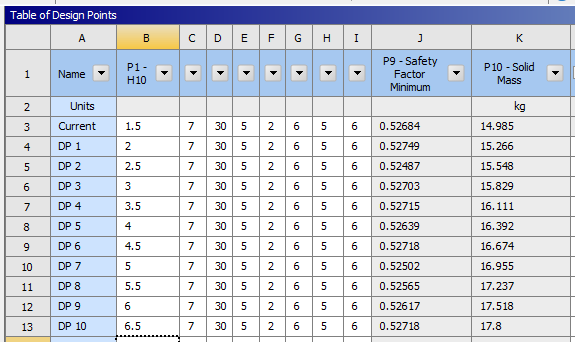
\includegraphics[width=0.75\textwidth]{singleParam/P1.PNG}

It can be seen that $H10$ can be reduced to save weight without decreasing safety factor greatly.
\item[P2] $=H11-H10$

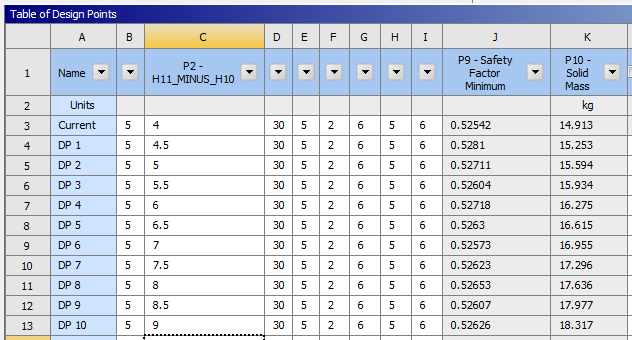
\includegraphics[width=0.75\textwidth]{singleParam/P2.PNG}

It can be seen that $H11$ can be reduced to save weight without decreasing safety factor greatly. Combined with the previous entry, we can seen that $H11$ can be reduced without decreasing safety factor greatly.
\item[P3] $=H1-H11$

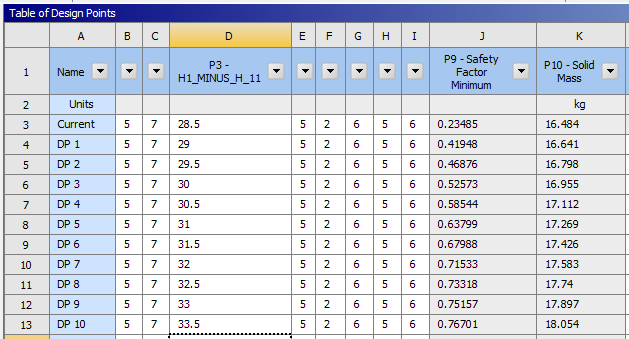
\includegraphics[width=0.75\textwidth]{singleParam/P3.PNG}

It can be seen that reducing $H1 - H11 - H9$, which is the part outer than the bearings, will reduce the safety factor greatly. That value should be increased instead.
\item[P4] $=V6$

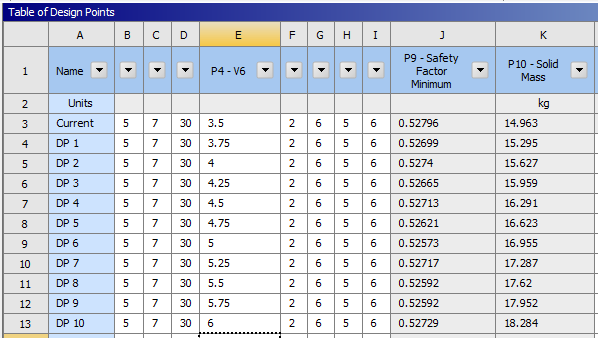
\includegraphics[width=0.75\textwidth]{singleParam/P4.PNG}

It can be seen that $V6$ can be reduced to save weight, and safety factor will not be influenced.
\item[P5] $=V3$

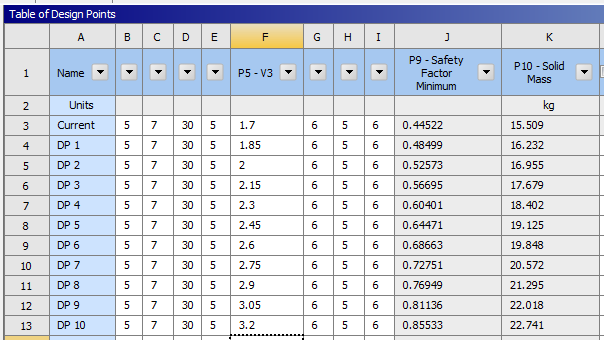
\includegraphics[width=0.75\textwidth]{singleParam/P5.PNG}

It can be seen that increasing $V3$ can increase the safety factor greatly.
\item[P7] $=HEIGHT / 2$

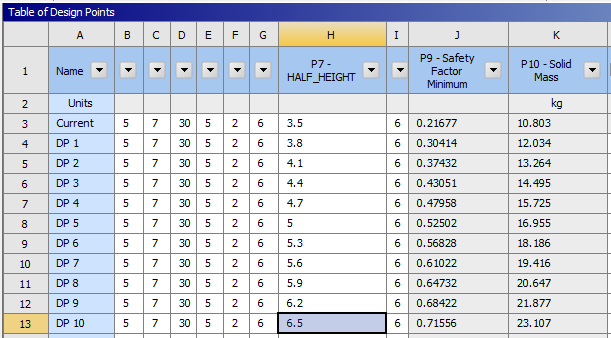
\includegraphics[width=0.75\textwidth]{singleParam/P7.PNG}

It can be seen that increasing the height will increase safety factor greatly. However, the weight will also be increased greatly.
\item[P8] $=D2$

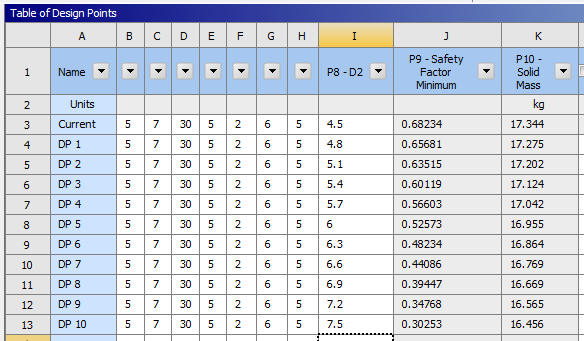
\includegraphics[width=0.75\textwidth]{singleParam/P8.PNG}

It can be seen that reducing $D2$ will increase the safety factor, and reduce the weight slightly. However, as reducing $D2$ will decrease the safety of the bolt significantly, it's preferred that $D2$ is kept at $6cm$ and not changed.
\end{description}
\subsubsection{Iteration 2}
As P5($V3$) is the most important factor, this time we only change P5.

According to the result of iteration 1, we try the following values will be used for other parameters:
\begin{align*}
P1 &= 1.5\\
P2 &= 4\\
P3 &= 33.5\\
P4 &= 3.5\\
P7 &= 4.7\\
P8 &= 6
\end{align*}

However, this resulted to stress concentration on the cylindrical surface of $D1$. 

TODO

\subsection{Automatic optimization}
The following settings will be used:

\begin{center}
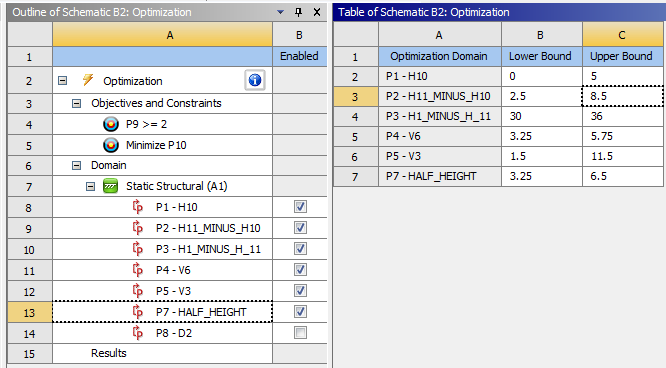
\includegraphics[width=0.75\textwidth]{OPT_BEFORE.PNG}
\end{center}

\section{Conclusion}
In this design project, the dimension of an anchor is optimized using ANSYS finite element analysis tool. 

We found that the maximum stress is likely to occur at four points, which are the side of the cylindrical surfaces for the bolt. We therefore optimize the design.

TODO
\end{document}